\documentclass[journal]{IEEEtran}
\usepackage{blindtext}
\usepackage{graphicx}
\usepackage[justification=centering]{caption}


\ifCLASSINFOpdf
  % \usepackage[pdftex]{graphicx}
  % declare the path(s) where your graphic files are
  % \graphicspath{{../pdf/}{../jpeg/}}
  % and their extensions so you won't have to specify these with
  % every instance of \includegraphics
  % \DeclareGraphicsExtensions{.pdf,.jpeg,.png}
\else
  % or other class option (dvipsone, dvipdf, if not using dvips). graphicx
  % will default to the driver specified in the system graphics.cfg if no
  % driver is specified.
  % \usepackage[dvips]{graphicx}
  % declare the path(s) where your graphic files are
  % \graphicspath{{../eps/}}
  % and their extensions so you won't have to specify these with
  % every instance of \includegraphics
  % \DeclareGraphicsExtensions{.eps}
\fi
% graphicx was written by David Carlisle and Sebastian Rahtz. It is
% required if you want graphics, photos, etc. graphicx.sty is already
% installed on most LaTeX systems. The latest version and documentation can
% be obtained at: 
% http://www.ctan.org/tex-archive/macros/latex/required/graphics/
% Another good source of documentation is "Using Imported Graphics in
% LaTeX2e" by Keith Reckdahl which can be found as epslatex.ps or
% epslatex.pdf at: http://www.ctan.org/tex-archive/info/
%

\begin{document}
\title{IS593 Term Project \emph{"Find Universal Cross Site Scripting Vulnerabilities in Brave Browser"}}

\author{Antoine RONDELET (20176461)}
\maketitle
\IEEEpeerreviewmaketitle

\section{Introduction}
Write the introduction at the end
Finish the introduction by a list of keywords.

It might be good to begin the paper with a bit of context about UXSS research. See whether we manage to find some papers about it -> if yes: speak about previous work, if no: speak about the fact that we couldn't find anything and that we were surprised to see that no previous work were carried out to try to study the security mechanisms of browsers and that current UXSS investigations are carried out by either companies themselves or by isolated persons reporting bugs to companies. This paper is an attempt to study browser's vulnerability, especially Universal XSS vulnerabilities.

\section{Web Browsers}

\subsection{Role}
Before presenting our work, we want to define what exactly a browser is and what is its intrinsic role. \\
According to Wikipedia, a web browser (commonly referred to as a browser) is a software application for retrieving, presenting and traversing information resources on the World Wide Web.\footnote{https://en.wikipedia.org/wiki/Web\_browser} 
While the primary role of these pieces of software is to provide an easy way for users to access web resources, most of today's web browsers implement a myriad of features such as the support for secure communications, the possibility to execute Javascript code or even the ability to be extended with plugins, to only name a few.

\begin{figure}[h]
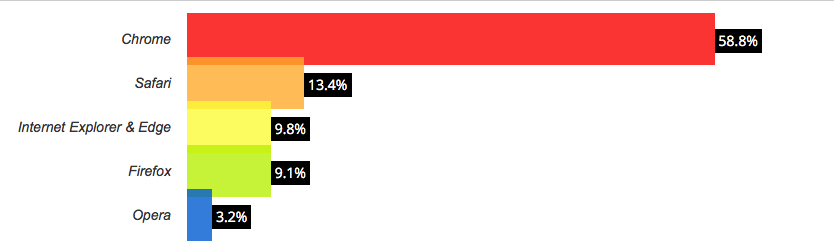
\includegraphics[width=0.4\textwidth]{images/WebBrowserMarketShare.png}
\caption{Web Browser Market Share in October 2017 \\ (from www.w3counter.com)}
\label{fig:marketShare}
\end{figure}

Around two decades after Netscape's Navigator and Window's Internet Explorer \emph{Browser wars}, the competition is still prevailing on the web browser market. The democratization of the use of the Web and, more recently, the introduction of HTML5, CSS3, and extensive client-side scripting to the World Wide Web, as well as more widespread use of smartphones and other mobile devices for browsing the web, lead to the apparition of dozens of browsers. From Mozilla's Firefox\footnote{https://www.mozilla.org/en-US/firefox/}, Google's Chrome\footnote{https://www.google.com/chrome/index.html}, Apple's Safari\footnote{https://www.apple.com/safari/} to Opera\footnote{http://www.opera.com/fr} for the most famous, the number of new browsers never ceases to increase. Today, as we are moving to the 4th industrial revolution - where data is moving astoundingly fast, and collected massively to be fed into \emph{Intelligent Agents} - some newcomers such as Brave\footnote{https://brave.com} or even Whale\footnote{http://whale.naver.com/en/} are trying to enter this disputed market and get their slice of the cake.
Although, figures \ref{fig:marketShare} and \ref{fig:monthlyUsage} agree on the fact that Google Chrome is the most widespread browser, other companies are working hard and hiring massively to try to dethrone Google's super star.

\begin{figure}[h]
\centering
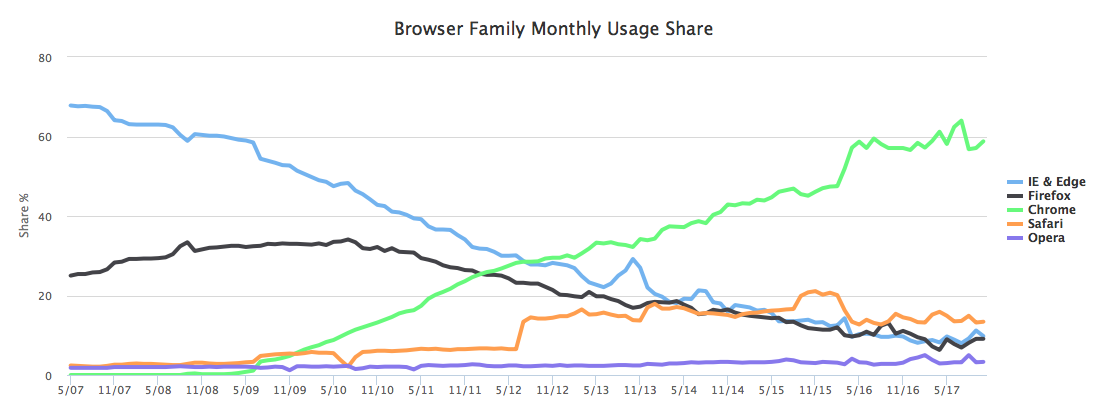
\includegraphics[width=0.4\textwidth]{images/BrowserFamilyMonthlyUsageShare.png}
\caption{Web Browser Monthly Usage Share \\ (from www.w3counter.com)}
\label{fig:monthlyUsage}
\end{figure}


As opposed to Netscape's Navigator, today, most web browsers are free to use. Developing web browsers is not about making money anymore, but more about sculpting people's computing habits in a way that would benefit the companies behind them.
As the market is quite competitive, developing a web browser can be seen as taking part into a race to developing the most features. This willingness to be different and attract people's attention often lead web browsers developers to implement features in a hurry. Such frequent releases sometimes unveil exploitable vulnerabilities and make browser's architecture more and more complex.

\medskip

A taste of a web browser's design is provided in the next part of this paper.

\subsection{Architecture}

Despite the large variety of browsers available to surf the web, they are almost all following a general structure. This architecture, as shown in \cite{architectureWebBrowsers} can be decomposed into eight components, each of which has its very own functionality.

\subsubsection{User Interface}
The component in charge of the UI contains every piece of the browser that is not actually part of the webpage itself. Such piece can either be toolbars or even previous and next buttons for instance.

\subsubsection{Browser Engine}
The browser engine forms the interface that allows the User Interface to interact and manipulate elements of the rendering engine.

\subsubsection{Rendering Engine}
The rendering engine is responsible for producing a graphical representation of the document fetched from a specific URL. It parses and render documents written in HTML and applies styles specified by CSS.

\subsubsection{Data Persistence}
The data persistence subsystem is responsible for insuring the persistence of data when the browser needs it. For instance, a browser needs to save data locally to keep track of the user's bookmarks and cookies.

\subsubsection{Networking}
Since a browser fetches document from the Web, a browser needs to be able to have an access to the network. This access is provided by the networking module. It implements file transfer protocols such as HTTP and FTP. Moreover, this subsystem translates between different character sets, and resolves MIME media types for files\footnote{https://en.wikipedia.org/wiki/Media\_type}. In some cases, the networking module might also implement a cache of recently retrieved resources to ensure good performances when a user asks multiple times the same resource.

\subsubsection{Javascript Interpreter}
This module interprets Javascript\footnote{Programming language developed by Netscape in 1995 to make webpages interactive. More details can be found at https://en.wikipedia.org/wiki/JavaScript} code

\subsubsection{XML parser}
The XML parser module is in charge of parsing XML documents into a Document Object Model (DOM) tree\footnote{https://en.wikipedia.org/wiki/Document\_Object\_Model}

\subsubsection{Display Backend}
The display backend subsystem provides primitives for drawing and windows. It also interfaces with the Operating System of the host machine.



\begin{figure}[h]
\centering
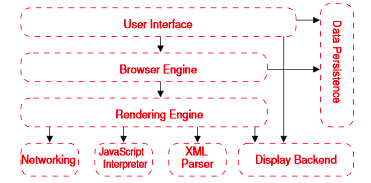
\includegraphics[width=0.4\textwidth]{images/BrowserStructure.png}
\caption{General Web Browser Structure}
\label{fig:browserStructure}
\end{figure}


\subsection{Security mechanisms}
\subsubsection{SoP}
\subsubsection{CORS}
\subsubsection{Sandboxes}
Speak about the role of sandboxes and speak about the difference between the security in Edge (window's side) and the google-chrome based browsers

\section{Brave}
Speak about the new features brought by Brave (speak about the company's policy to ensure privacy on the web and so on...) + the BAT principle and the new things that are brought by Brave and why we decided to study this web browser in particular
+ Speak about other new browsers such as Whale and so on just to show that many actors are actually trying to take Google Chrome's market share.

\section{Universal XSS}
Describe what Universal XSS is, and explain the consequences it has.

\section{Previous attacks and patterns used to defeat the security mechanisms of web browsers}
Today web browsers are extremely complicated pieces of software (speak about complex architecture described in the section above). So there are potential vulnerabilities that escaped to the development teams and can be used by malicious users.

\medskip

Speak about the patterns we found in the different attack report we studied (CVE and Broken Browser and so on)

\section{Our attempts}
Say that none of our attempts were successful but that we provide them as a record of our work. They might also be extended/adapted to carry out successful attack.

\medskip

Speak about what we tried, and why we tried it, and explain what we had in mind when we tried something (so that the reader can understand the attack more easily)

\medskip

Conclude this section by saying that today's browsers are not trivially vulnerable (fortunately), however it is not because we didn't manage to find a vulnerability that no one is going to find one.

\section{Conclusion}
Despite the fact that we didn't manage to find any vulnerability on the web browsers, some persons might be able to find some. It is important to remember that browsers act as a last rampart against malicious users/attackers. As many browsers are on the market today, the teams developing them are in a perpetual race against each other. The best browser is the most secure one with the most features to provide their users. However, as features are added to a browser, it is paramount to keep in mind the aspect of security.

\section{IDEAS for the paper}



% if have a single appendix:
%\appendix[Proof of the Zonklar Equations]
% or
%\appendix  % for no appendix heading
% do not use \section anymore after \appendix, only \section*
% is possibly needed

% use appendices with more than one appendix
% then use \section to start each appendix
% you must declare a \section before using any
% \subsection or using \label (\appendices by itself
% starts a section numbered zero.)
%

% Can use something like this to put references on a page
% by themselves when using endfloat and the captionsoff option.

\begin{thebibliography}{1}

\bibitem{website}
https://www.brokenbrowser.com/uxss-edge-domainless-world/

\bibitem{paper1}
MJ Rees
\textit{Evolving the Browser Towards a Standard User Interface Architecture}, 2001

\bibitem{architectureWebBrowsers}
Alan Grosskurth, and Michael W. Godfrey
\textit{A reference architecture for web browsers}, 2006

\end{thebibliography}

\ifCLASSOPTIONcaptionsoff
  \newpage
\fi



% trigger a \newpage just before the given reference
% number - used to balance the columns on the last page
% adjust value as needed - may need to be readjusted if
% the document is modified later
%\IEEEtriggeratref{8}
% The "triggered" command can be changed if desired:
%\IEEEtriggercmd{\enlargethispage{-5in}}

% references section

% can use a bibliography generated by BibTeX as a .bbl file
% BibTeX documentation can be easily obtained at:
% http://www.ctan.org/tex-archive/biblio/bibtex/contrib/doc/
% The IEEEtran BibTeX style support page is at:
% http://www.michaelshell.org/tex/ieeetran/bibtex/
%\bibliographystyle{IEEEtran}
% argument is your BibTeX string definitions and bibliography database(s)
%\bibliography{IEEEabrv,../bib/paper}
%
% <OR> manually copy in the resultant .bbl file
% set second argument of \begin to the number of references
% (used to reserve space for the reference number labels box)

% biography section
% 
% If you have an EPS/PDF photo (graphicx package needed) extra braces are
% needed around the contents of the optional argument to biography to prevent
% the LaTeX parser from getting confused when it sees the complicated
% \includegraphics command within an optional argument. (You could create
% your own custom macro containing the \includegraphics command to make things
% simpler here.)
%\begin{biography}[{\includegraphics[width=1in,height=1.25in,clip,keepaspectratio]{mshell}}]{Michael Shell}
% or if you just want to reserve a space for a photo:

% You can push biographies down or up by placing
% a \vfill before or after them. The appropriate
% use of \vfill depends on what kind of text is
% on the last page and whether or not the columns
% are being equalized.

%\vfill

% Can be used to pull up biographies so that the bottom of the last one
% is flush with the other column.
%\enlargethispage{-5in}



% that's all folks
\end{document}


